\documentclass[a4paper,11pt]{article}
\usepackage{amsmath,amsthm,amsfonts,amssymb,amscd,amstext,vmargin,graphics,graphicx,tabularx,multicol} 
\usepackage[francais]{babel}
\usepackage[utf8]{inputenc}  
\usepackage[T1]{fontenc} 
\usepackage{pstricks-add,tikz,tkz-tab,variations}
\usepackage[autolanguage,np]{numprint} 
\usepackage{color}

\setmarginsrb{1.5cm}{0.5cm}{1cm}{0.5cm}{0cm}{0cm}{0cm}{0cm} %Gauche, haut, droite, haut
\newcounter{numexo}
\newcommand{\exo}[1]{\stepcounter{numexo}\noindent{\bf Exercice~\thenumexo} : \marginpar{\hfill /#1}}
\reversemarginpar


\newcounter{enumtabi}
\newcounter{enumtaba}
\newcommand{\q}{\stepcounter{enumtabi} \theenumtabi.  }
\newcommand{\qa}{\stepcounter{enumtaba} (\alph{enumtaba}) }
\newcommand{\initq}{\setcounter{enumtabi}{0}}
\newcommand{\initqa}{\setcounter{enumtaba}{0}}

\newcommand{\be}{\begin{enumerate}}
\newcommand{\ee}{\end{enumerate}}
\newcommand{\bi}{\begin{itemize}}
\newcommand{\ei}{\end{itemize}}
\newcommand{\bp}{\begin{pspicture*}}
\newcommand{\ep}{\end{pspicture*}}
\newcommand{\bt}{\begin{tabular}}
\newcommand{\et}{\end{tabular}}
\renewcommand{\tabularxcolumn}[1]{>{\centering}m{#1}} %(colonne m{} centrée, au lieu de p par défault) 
\newcommand{\tnl}{\tabularnewline}

\newcommand{\bmul}[1]{\begin{multicols}{#1}}
\newcommand{\emul}{\end{multicols}}

\newcommand{\trait}{\noindent \rule{\linewidth}{0.2mm}}
\newcommand{\hs}[1]{\hspace{#1}}
\newcommand{\vs}[1]{\vspace{#1}}

\newcommand{\N}{\mathbb{N}}
\newcommand{\Z}{\mathbb{Z}}
\newcommand{\R}{\mathbb{R}}
\newcommand{\C}{\mathbb{C}}
\newcommand{\Dcal}{\mathcal{D}}
\newcommand{\Ccal}{\mathcal{C}}
\newcommand{\mc}{\mathcal}

\newcommand{\vect}[1]{\overrightarrow{#1}}
\newcommand{\ds}{\displaystyle}
\newcommand{\eq}{\quad \Leftrightarrow \quad}
\newcommand{\vecti}{\vec{\imath}}
\newcommand{\vectj}{\vec{\jmath}}
\newcommand{\Oij}{(O;\vec{\imath}, \vec{\jmath})}
\newcommand{\OIJ}{(O;I,J)}


\newcommand{\reponse}[1][1]{%
\multido{}{#1}{\makebox[\linewidth]{\rule[0pt]{0pt}{20pt}\dotfill}
}}

\newcommand{\titre}[5] 
% #1: titre #2: haut gauche #3: bas gauche #4: haut droite #5: bas droite
{
\noindent #2 \hfill #4 \\
#3 \hfill #5

\vspace{-1.6cm}

\begin{center}\rule{6cm}{0.5mm}\end{center}
\vspace{0.2cm}
\begin{center}{\large{\textbf{#1}}}\end{center}
\begin{center}\rule{6cm}{0.5mm}\end{center}
}



\begin{document}
\pagestyle{empty}
\titre{Interrogations sur le théorème de Thalès et sa réciproque }{Nom :}{Prénom :}{Classe}{Date}

\begin{flushleft}
\begin{tabular}{|m{9.5cm}|m{1.25cm}|m{1.25cm}|m{1.25cm}|m{1.25cm}|m{1.25cm}|}
\hline 
\textbf{Compétences} & \begin{center}
\textbf{N.E.}
\end{center} & \begin{center}
\textbf{M.I.}
\end{center} & \begin{center}
\textbf{M.F.}
\end{center}  & \begin{center}
\textbf{M.S.}
\end{center} & \begin{center}
\textbf{T.B.M.}
\end{center} \\ 
\hline 
Je dois connaître et savoir utiliser le théorème de Thalès pour calculer une longueur &  &  & & &\\
\hline 
JJe dois connaître et savoir utiliser la réciproque du théorème de Thalès &  &  & & &\\
\hline


\end{tabular} 
\end{flushleft}

\textit{N.E = Non évalué ; M.I. = Maîtrise insuffisante ; M.F. = Maîtrise fragile ; M.S. = Maîtrise satisfaisante ; T.B.M. = Très bonne maîtrise}\\


\vspace*{0.3cm}

\exo{4} Sur la figure suivante, les droites (ED), (GF) et (AC) sont parallèles.

\begin{center}
\includegraphics[scale=0.8]{thales6.eps} 
\end{center}

\q Calculer AC.\\
\reponse[10]\\


\q Calculer FG.\\
\reponse[10]\\



\exo{3}

\noindent Dans les marais salants, le sel récolté est stocké sur une surface plane.\\
On admet qu'un tas de sel a toujours la forme d'un cône de révolution.\\
Pascal souhaite déterminer la hauteur d'un cône de sel de diamètre 5 mètres. Il possède un bâton de longueur 1 mètre. Il effectue des mesures et réalise les deux schémas ci-dessous.\\


\includegraphics[scale=1]{thales2.eps} 





\initq \q Démontrer que la hauteur de ce cône de sel est égale à 2,5 mètres\\
\reponse[12]\\

\exo{3}  Le dessin ci-dessous est un schéma d'une table à repasser en cm.\\ Cette table à repasser est-elle parallèle au sol ? Justifier votre réponse.

\begin{center}
\includegraphics[scale=0.8]{thales7.eps} 
\end{center}

\noindent \reponse[9]\\

\vspace*{0.5cm}

\exo{Bonus}

On considère la figure ci-dessous sur laquelle:\\

AN est le plus grand des facteurs premiers de la décomposition de 231\\

$AC = \dfrac{2 ^ {3} \times 5 \times 11}{8}  $\\

AM est le plus grand des diviseurs de 30 (excepté 30)\\

AB est le PGCD de 1 500 et 11 025  \\


%AN = 11
%AC = 55
%MN = 
%AB = 75
%AM = 15

\begin{center}
\includegraphics[scale=0.8]{thales3_cas_simple.eps} 
\end{center}

\initq \q Démontrer que les droites (MN) et (BC) sont parallèles.\\

\noindent \reponse[9]\\

\end{document}
